\section{Configuration and Control of Experiments}
\label{sec:confandControl}
Software experiments that do not require interacting directly with humans (e.g., through graphic user interfaces (GUI) or Human–computer interaction software (HCI)) are not strongly influenced by human factors (e.g., personality, preferences, human environment, education, age, culture, among others). However, there are related variables that must be configured to ensure that they won't affect the experiments results. These configurations are realized to guarantee the experiments reliability and it is also known as calibration. Additionally, they are accompanied by experiments rehearsals. It is important to guarantee that there are no unidentified variables that affect the results of the experiments before starting the experiments execution. In this case, these variables refer to the configuration of experiments, including, the Precision Time Protocol (PTP), the Java version and the Java Virtual Machine (JVM) configuration, the software deployment configuration, the operating system, and the hardware configuration. Some of these variables were described in section \ref{sec:contextVariablesSearch} showing their importance on systems performance. However, in our case, we do not vary their values to determine how they affect performance. We only select one configurable value to each one to control how they affect system performance with these definitions and values, we performed pilot experiments to calibrate and tune the chosen values that allow us to guarantee that these variables configuration and the unidentified variables do not affect the experiments. 

\subsection{Hardware Configuration}
Experiments were executed out in the LIASOn laboratory of the Universidad Icesi. This laboratory has 18 computers that are used as processing nodes, a Network Attached Storage (NAS) that allows information to be shared among processing nodes, and its own private network, through a 10 Gbps switch with 24 ports. Table \ref {tab:hardware_config} summarizes characteristics of the device types. 

\begin{table}[]
	\centering
	\caption{Hardware Configuration}
	\label{tab:hardware_config}
	 \resizebox{\textwidth}{!}{%
	\begin{tabular}{|c|c|c|c|c|c|}
		\hline
		\textbf{DEVICE}                                                               & \textbf{NAME}                                                              & \textbf{PROCESSOR}                                                              & \textbf{\begin{tabular}[c]{@{}c@{}}OPERATING\\ SYSTEM\end{tabular}}                       & \textbf{MEMORY}       & \textbf{HDD}       \\ \hline
		\begin{tabular}[c]{@{}c@{}}Processing \\ Nodes (18) \end{tabular}                                                                            & \begin{tabular}[c]{@{}c@{}}DELL \\ OPTIPLEX 7010\end{tabular}              & \begin{tabular}[c]{@{}c@{}}Intel Core i7 - 3770 \\ @3.40Ghz (4 physical cores)\end{tabular}        & \begin{tabular}[c]{@{}c@{}}Fedora 21 \\ 64 bits\end{tabular}                              & 16 GB                 & 320 GB             \\ \hline
		\multicolumn{6}{|c|}{}                                                                                                                                                                                                                                                                                                                                                                \\ \hline
		\begin{tabular}[c]{@{}c@{}}Network\\   Attached \\ Storage (NAS) (1)\end{tabular} & \begin{tabular}[c]{@{}c@{}}Dell Power \\ Vault NX400\end{tabular}          & \begin{tabular}[c]{@{}c@{}}Intel ® Xeon\\   ® E5-2403 \\ Quad Core\end{tabular} & \begin{tabular}[c]{@{}c@{}}Microsoft Windows\\     Storage Server \\ 2012 R2\end{tabular} & 18 GB                 & 4 TB               \\ \hline
		\multicolumn{2}{|c|}{}                                                                                                                                     & \multicolumn{2}{c|}{\textbf{SUPPORTED TRANSMISSION RATE}}                                                                                                                            & \multicolumn{2}{c|}{\textbf{PORTS}} \\ \hline
		Switch (1)                                                                        & \begin{tabular}[c]{@{}c@{}}Dell Networking\\     N4000 Series\end{tabular} & \multicolumn{2}{c|}{10/100/1000/10000  (Mb/s)}                                                                                                                              & \multicolumn{2}{c|}{24}                    \\ \hline
	\end{tabular}%
}
\end{table}

\subsection{Operating System Configuration}
As we mentioned in section \ref{sec:contextVariablesSearch}, the operating system can affect the system performance given that it is responsible to manage hardware resources through daemon processes and user processes and provide services to applications to access or use the hardware resources. In our experiments, all processing nodes have Fedora 21 operating system (64 bits). Its daemon processes serves main functions, not all of them required for executing the experiments, thus, we  analyze which of these processes are needed during our experiments execution and we developed a script to shutdown unnecessary processes that the operating system might start. The objective of this script is to minimize the possibility that one of these processes may affect the experiments using resources for other tasks outside of our experiments. To develop the script, we explored one by one each of them and determined if our application or operating system required this service or process. (The script is presented in Appendix A - section \ref{sec:appendA}).

\subsection{Precision Time Protocol (PTP)}
Precision Time Protocol (PTP) is a software implementation of the IEEE standard 1588 for Linux. In this thesis, this protocol has a special role because for taking measurements in distributed environments requires synchronization among processing nodes. For example, when we measure communication time, this time has to be collected in two different nodes (sender and receiver). The communication time is calculated as the difference between the instant the message is received (time in milliseconds) minus the instant the message is sent (time in milliseconds). If nodes are not synchronized, this measurement is not accurate. This protocol allows a precision in nanoseconds, and measurements are taken in milliseconds, so it fulfills the measurement requirements. 


\subsection{Other Software and their Configurations}
Other variables that also must be configured are the instrumentation variables. These are the ones that are used to execute the experiments, for example,  middle-ware and support software. These variables can affect the experiments results through their own values and procedures of configuration, or the used version, because depending on them each application can change the way to manage its resources, and therefore they affect the system performance. The following are the software versions and their configuration used during experiments.

\begin{description}
	\item [FraSCAti:] This software is used to support SCA component implementation. We use Frascati version 1.4 because it was the most stable version available.
	\item [Ice:] This software is used to support the communication between distributed components. We use Ice version 3.5.
	\item [Java:] All code of the applications to execute the experiments was implemented in java. We use Java version 1.6 Update 23 because it is the most compatible with FraSCAti.
	\item [Tomcat:] This is used as a server application facade when we use Ice because the basic version of Ice does not manage REST requests. We use Tomcat version 8.
	\item [Jmeter:] This is used to simulate user requests. We used Jmeter version 2.13.
	\item [RabbitMQ:] This is used by PaSCAni library to send and take measurements to probes.  We used RabbitMQ version 3.6 (Configuration is presented in section \ref{sec:appendB} - Appendix B).
	\item [Java Virtual Machine (JVM) Configuration:] Java Virtual Machine configuration can affect experiments. However, we only focus on maximum and minimum memory configuration. Memory size can affect the experiments directly given the size of the files that have to be sorted. We configured the JVM memory to 6 GB (Configuration is presented in section \ref{sec:appendC} - Appendix C).
	
\end{description}


\section{Software Deployment Configuration}
Amelia is a library developed by Miguel Jimenez \cite{AmeliaMiguelJimenez} to automate the deployment of distributed component-based software. Using this library, we implemented classes to automate the execution of experiment designed in chapter \ref{cha:experimentDesign}. In the next sections, we present the deployment diagrams for the sorting software for all design pattern and strategies variation that we used as architectural guides to implement the required classes, as their deployment specification.

\subsubsection{JC Sorting Strategy}
\label{subsubsec:ameliaOriginalStrategy}
This strategy consists in splitting the input data recursively to halves while there are available processing nodes. For example, for 4 available nodes configuration (cf. figure \ref{fig:diagramJCMunozOriStr})  and a file size of 1'600.000 lines. First node splits the input data to half (800.000 lines), it keeps one half to process and sends the other half to its son, in the next higher hierarchical level. Its son splits input data again (400.000), and  sends to its son one half, and processes the other half. To continue with first node, it splits data again (400.000) and it sends to its other son one half, and it processes the remaining.

Figure \ref{fig:diagramJCMunozOriStr} shows the deployment diagram used to develop the amelia deployment automation classes. Almost all controllable variable combinations generate a new Amelia deployment classes, except the File Size and the Bandwidth variables. For these two variables, the amelia deployment classes can be reused using parameters. However, deployment diagrams only vary according to available processing nodes variable. This variable can take the next values: 1, 2, 4, 8, and 16 as established in the experiment design (cf. section \ref{sec:benchmark}). The presented diagram corresponds to the 8 nodes configuration. This diagram can be used to visualize all other configurations. 

To visualize the 2 nodes configuration, the processing nodes Hgrid1 and Hgrid5 are used to sort the input file. The 4 nodes configuration, Hgrid3 and Hgrid6 are added as processing nodes. To visualize the 16 nodes configuration the idea is to connect Hgrid1 with an additional node, and this new node has the same hierarchical structure of Hgrid1 in 8 nodes configuration (i.e., recursively). 

The Hgrid9 is not a processing node. It has components needed to take measurements and make reports. Hgrid17 is neither a processing node: it has components needed to automate experiments and the RabbitMq Server to support the measurements message passing. Nodes Hgrid9 and Hgrid17 remains the same through all experiments configuration.


\begin{landscape}
	\begin{figure}[p!]
		\centering
		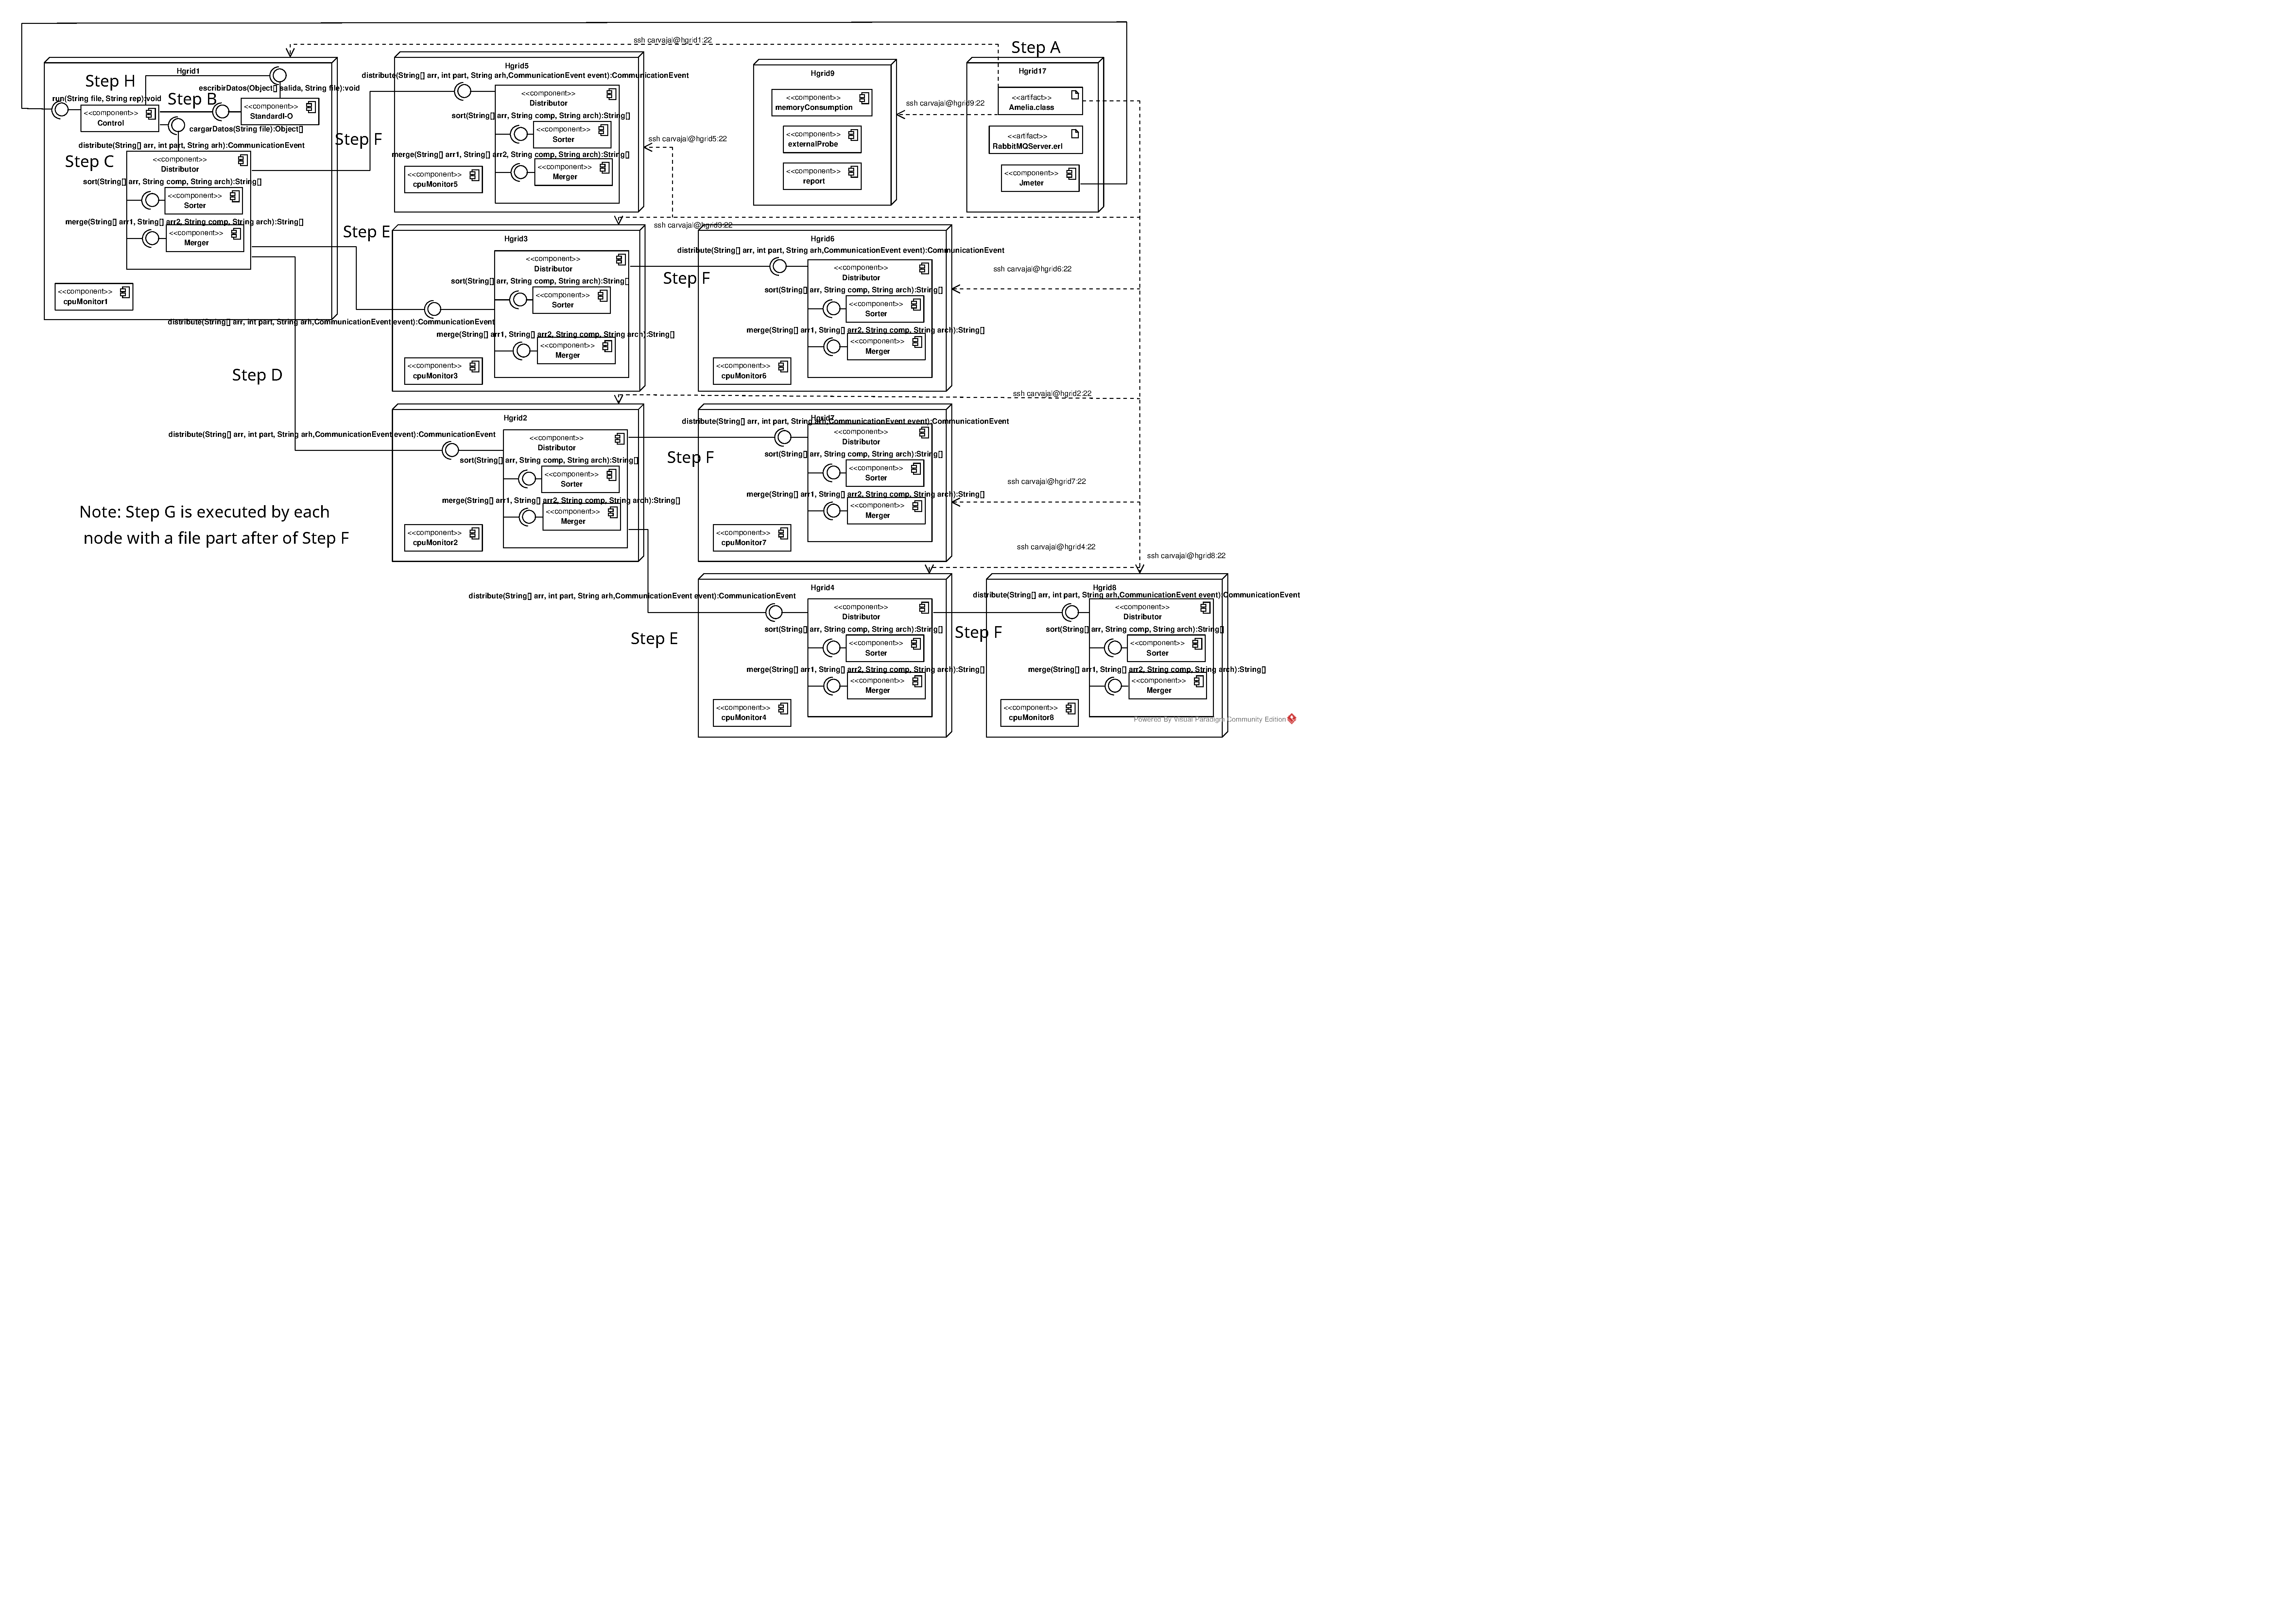
\includegraphics[trim=4cm 45cm -4cm 2cm, scale=0.4]{fig/JCMunozOriginalStrategy.pdf}
		\caption{Amelia - Deployment Diagram - The JC Sorting Strategy}
		\label{fig:diagramJCMunozOriStr}
	\end{figure}
	
\end{landscape}

The behavior of the JC Sorting Strategy is described next:\\

\begin{description}
	\item [Step A] The Jmeter component of processing node Hgrid17 starts processing when it calls the run method of the control component (processing node Hgrid1).
	\item [Step B] The control component sends to the StandardI-O component a read request to load the input file.
	\item [Step C] The control component sends to the Distributor component in Hgrid1 a distribute request with the whole input file as parameter.
	\item [Step D] The Distributor component of Hgrid1 sends to the Distributor component in Hgrid2 a distribute request with the half of the input file.
	\item [Step E] In this step two requests are sent in parallel. The Distributor component of Hgrid1 sends to the Distributor component in Hgrid3 a distribute request with a 1/4 of the input file and the Distributor component of Hgrid2 sends to the Distributor component in Hgrid4 a distribute request with a 1/4 of the input file.
	\item [Step F] In this step four request are sent in parallel. (i) The Distributor component of Hgrid1 sends to the Distributor component in Hgrid5 a distribute request with a 1/8 of the input file; (ii) the Distributor component of Hgrid2 sends to the Distributor component in Hgrid7 a distribute request with a 1/8 of the input file; (iii) the Distributor component of Hgrid4 sends to the Distributor component in Hgrid8 a distribute request with a 1/8 of the input file; and (iv) the Distributor component of Hgrid3 sends to the Distributor component in Hgrid6 a distribute request with a 1/8 of the input file.
	\item [Step G] All processing nodes sort their file part and return each sorted file part to their own father processing node, which merges the file parts.
	\item [Step H] The control component receives the whole sorted file and it sends a write request to the StandardI-O component.
\end{description}


\subsubsection{Variant of the JC Sorting Strategy - Separation of Merge Component}
This variant is illustrated in Fig. \ref{fig:diagramJCMunozMergerSeparated}. It applies the same configuration used in the previous diagram (cf. Figure \ref{fig:diagramJCMunozOriStr}), with the only difference that there is only one merge component. The merge component is located in the processing node Hgrid1. We proposed this difference for the merge solution must have complexity of O(n) and it can be incremented because of amount the recursive merge stages, therefore, we calculate that the performance can be improved if there is only one merge phase because in the JC sorting strategy there are more than one merge of the same data.

\begin{landscape}
	\begin{figure}[p!]
		\centering
		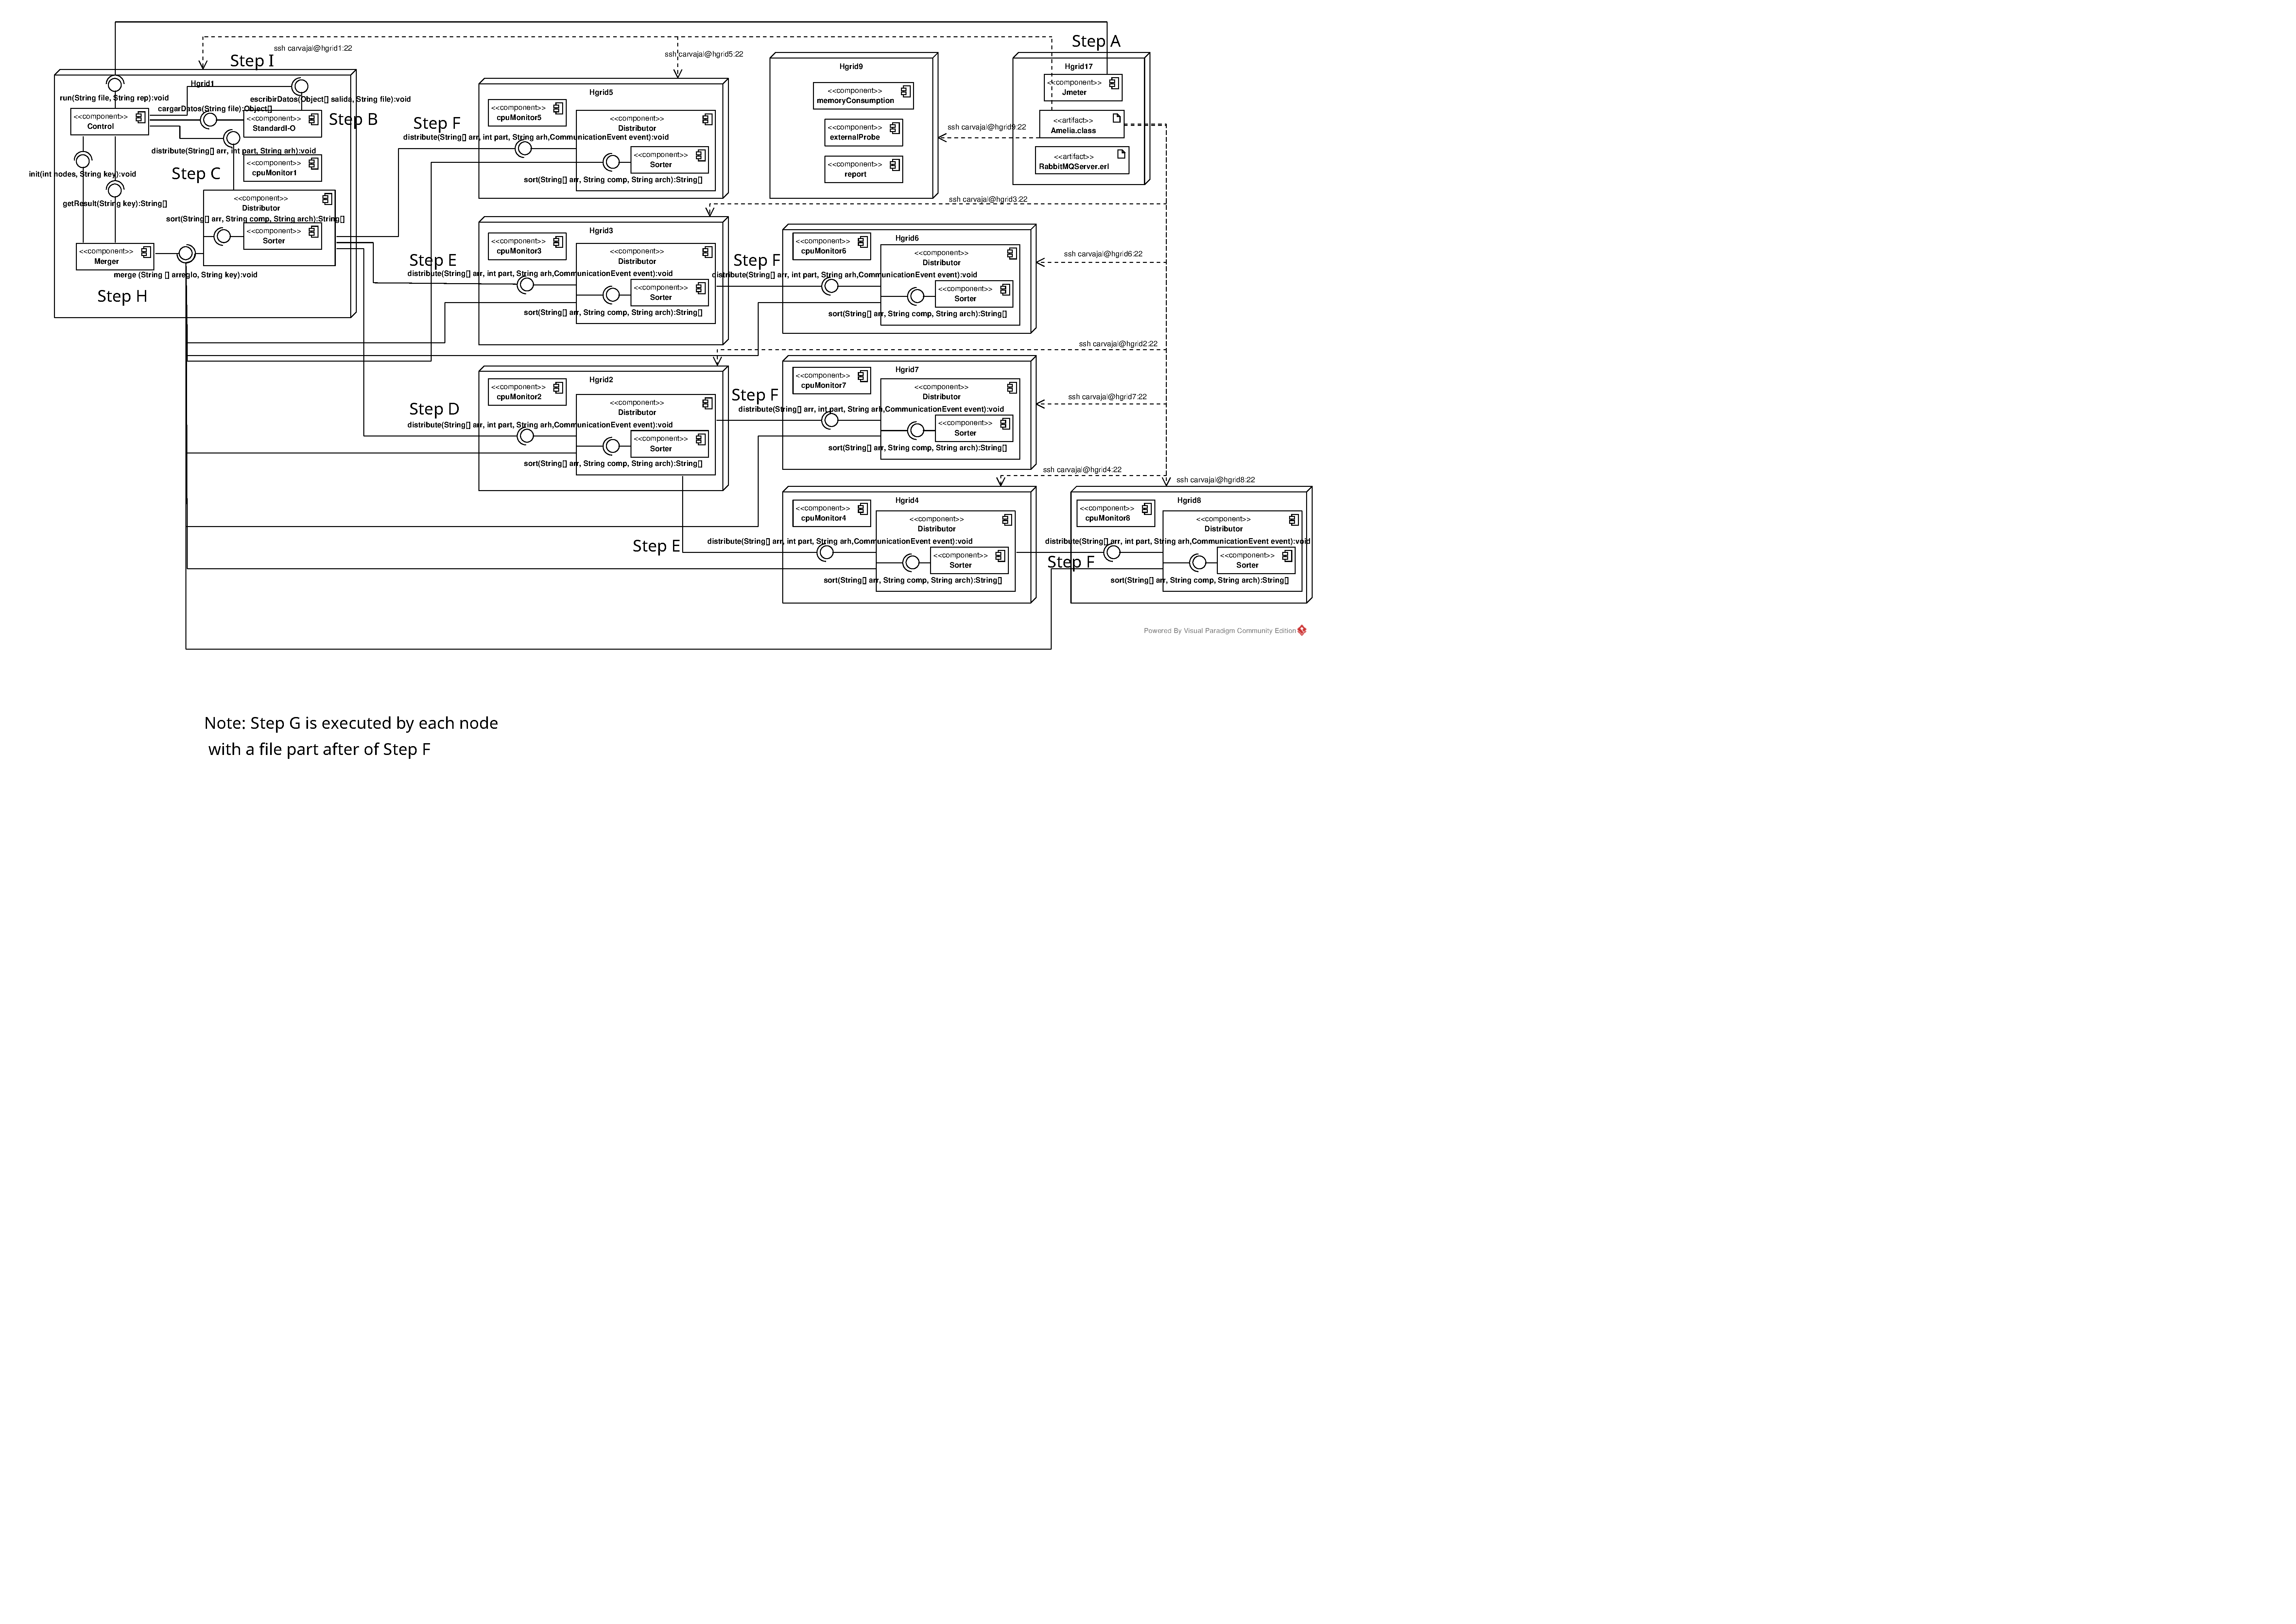
\includegraphics[trim=6cm 45cm -6cm 2cm, scale=0.4]{fig/JCMunozMergerSeparated.pdf}
		\caption{Amelia - Deployment Diagram - Variant of the JC Sorting Strategy - Separation of Merge Component}
		\label{fig:diagramJCMunozMergerSeparated}
	\end{figure}
	
\end{landscape}

The behavior of the Variant of the JC Sorting Strategy is described next:

\begin{description}
	\item [Step A] The Jmeter component of the processing node Hgrid17 starts processing when it calls the run method of the control component (processing node Hgrid1).
	\item [Step B] The control component sends to the StandardI-O component a read request to load the input file.
	\item [Step C] The control component sends to the Distributor component in Hgrid1 a distribute request with the whole input file as parameter.
	\item [Step D] In this step two request are sent in parallel. The Distributor component of Hgrid1 sends to the Distributor component in Hgrid2 a distribute request with the half of the input file and the control component initializes the merger component.
	\item [Step E] In this step three request are sent in parallel. (i) The Distributor component of Hgrid1 sends to the Distributor component in Hgrid3 a distribute request with a 1/4 of the input file; (ii) the Distributor component of Hgrid2 sends to the Distributor component in Hgrid4 a distribute request with a 1/4 of the input file; and (iii) the control component sends to the merger component a request to get the whole sorted file when all file parts will be merged.
	\item [Step F] In this step four request are sent in parallel. (i) The Distributor component of Hgrid1 sends to the Distributor component in Hgrid5 a distribute request with a 1/8 of the input file; (ii) the Distributor component of Hgrid2 sends to the Distributor component in Hgrid7 a distribute request with a 1/8 of the input file; (iii) the Distributor component of Hgrid4 sends to the Distributor component in Hgrid8 a distribute request with a 1/8 of the input file; and (iv) the Distributor component of Hgrid3 sends to the Distributor component in Hgrid6 a distribute request with a 1/8 of the input file.
	\item [Step G] All processing nodes sort their file part and send a merger request to the merger component with their own sorted file part.
	\item [Step H] The merger component receives all sorted file parts, and merges them and answers to the control component the request realized in Step E.
	\item [Step I] The control component receives the whole sorted file and it sends a write request to the StandardI-O component.
\end{description}

\subsubsection{Fork/Join Java library}
This variant uses the same deployment diagram used for the previous variant. However, it differs to the previous because it implements Java Fork-Join library in each node to process its own file chunk.

\subsubsection{Fork-Join Design Pattern}
The JC sorting strategy introduces latency given its hierarchical structure. By applying the Fork/Join pattern we can avoid this added latency. To implement this design pattern in a distributed deployment we need to answer two questions:
 \begin{itemize}
 	\item Which is the minimum chunk size worth if distributing the computations?
 	\item How many available nodes (children) should have each processing node to distribute?
 \end{itemize}
  
  The first question focuses on cases where distribution is not cost effective because distribution implies performance loss due to latency addition. The second question is focused on managing the processing nodes. The Fork/Join Java library leaves this task to the operating system through CPU core assignment. However, in a distributed deployment we must decide how processing nodes are assigned. We identify two options (i) only one node can execute forks and it has all available processing nodes associated to it; and (ii) all nodes can execute forks, but each one has a limited amount of processing nodes associated to it. When this amount is reached, if there appear a new available node it is assigned to next level of processing nodes (children of children, that is, grandchildren). For example, assuming that the limited amount is three nodes, if the first node has three associated nodes and there is a new available node, this node would be associated with any of the three children of the first node.

We will analyze the answer to the first question in the next section (cf. section \ref{sec:prepExperiments}) because in this section we will realize tests through preparatory experiments to decide which will be the minimum chunk size.
% results of experiments consolidated in table \ref{tab:mimfileSizeEx}. We decide take as minimum size to fork 400.000 lines because it is possible to observe that 200.000 lines and 600.000 lines can leverage distribution, therefore we calculate average between these values. Additionally we can observe that difference between 1 and 2 nodes for 400.000 lines is small.

To answer the second question, where we need to define how many children nodes can have each node, we try to select a behavior similar to the used in the JC sorting strategy to increase comparability. According to this, the second option (ii) exposed before, where all nodes will have the capacity of executing forks, is more appropriate. In this option we can distribute in a similar way that the JC sorting strategy, but the hierarchical structure will be more homogeneous, besides avoiding performance loss added by the added latency in the hierarchy when more nodes are added. The maximum amount of processing nodes associated to each node was defined in 3 because it can support the maximum amount of processing nodes defined for our experiments (16).

Figure \ref{fig:diagramJCMunozDistributedFJ} shows the deployment diagram of this configuration for 8 nodes.

The Fork-Join Design Pattern behavior is described as follows:

\begin{description}
	\item [Step A] The Jmeter component of the processing node Hgrid17 starts processing when it calls the run method of the control component (processing node Hgrid1).
	\item [Step B] The control component sends to the StandardI-O component a read request to load the input file.
	\item [Step C] The control component sends to the Distributor component in Hgrid1 a distribute request with the whole input file as parameter.
	\item [Step D] In this step the merger component is initialized and the first level of distributors are called in parallel. The Distributor component of Hgrid1 sends to the Distributor components in Hgrid2, Hgrid3 and Hgrid4 a distribute request with a 1/4 of the input file.
	\item [Step E] In this step some requests are sent in parallel: (i) The Distributor components in Hgrid2, Hgrid3 and Hgrid4 send to their own children Distributor components in Hgrid6, Hgrid7, Hgrid10 and Hgrid13 a distribute request with a 1/8 of the input file; (ii) the Distributor component in Hgrid1 starts to sort its file part. First, it divides its file part in more little chunks (these chunks depend on the CPU amount of each node, in our case each node divides its file part into 8 parts) to apply the Fork/Join Java library and to have work if any of its children will finish processing before and so help it. When this component finishes to process each file part, it sends a merger request to the merger component with its own sorted file parts; and (iii) the control component sends to the merger component a request to get the whole sorted file when all file parts will be merged.
	\item [Step F] In this step all Distributor components start to sort their file part, in the same way that the Distributor component in Hgrid1 did in the step E. When any of the sorter components finishes their work, it verifies if it can help its father node or the work have been finished.
	\item [Step G] The merger component receives all sorted file parts, it merges the whole sorted file and answers to the control component the request realized in Step E.
	\item [Step H] The control component receives the whole sorted file and it sends a write request to the StandardI-O component.
\end{description}

\begin{landscape}
	\begin{figure}[p!]
		\centering
		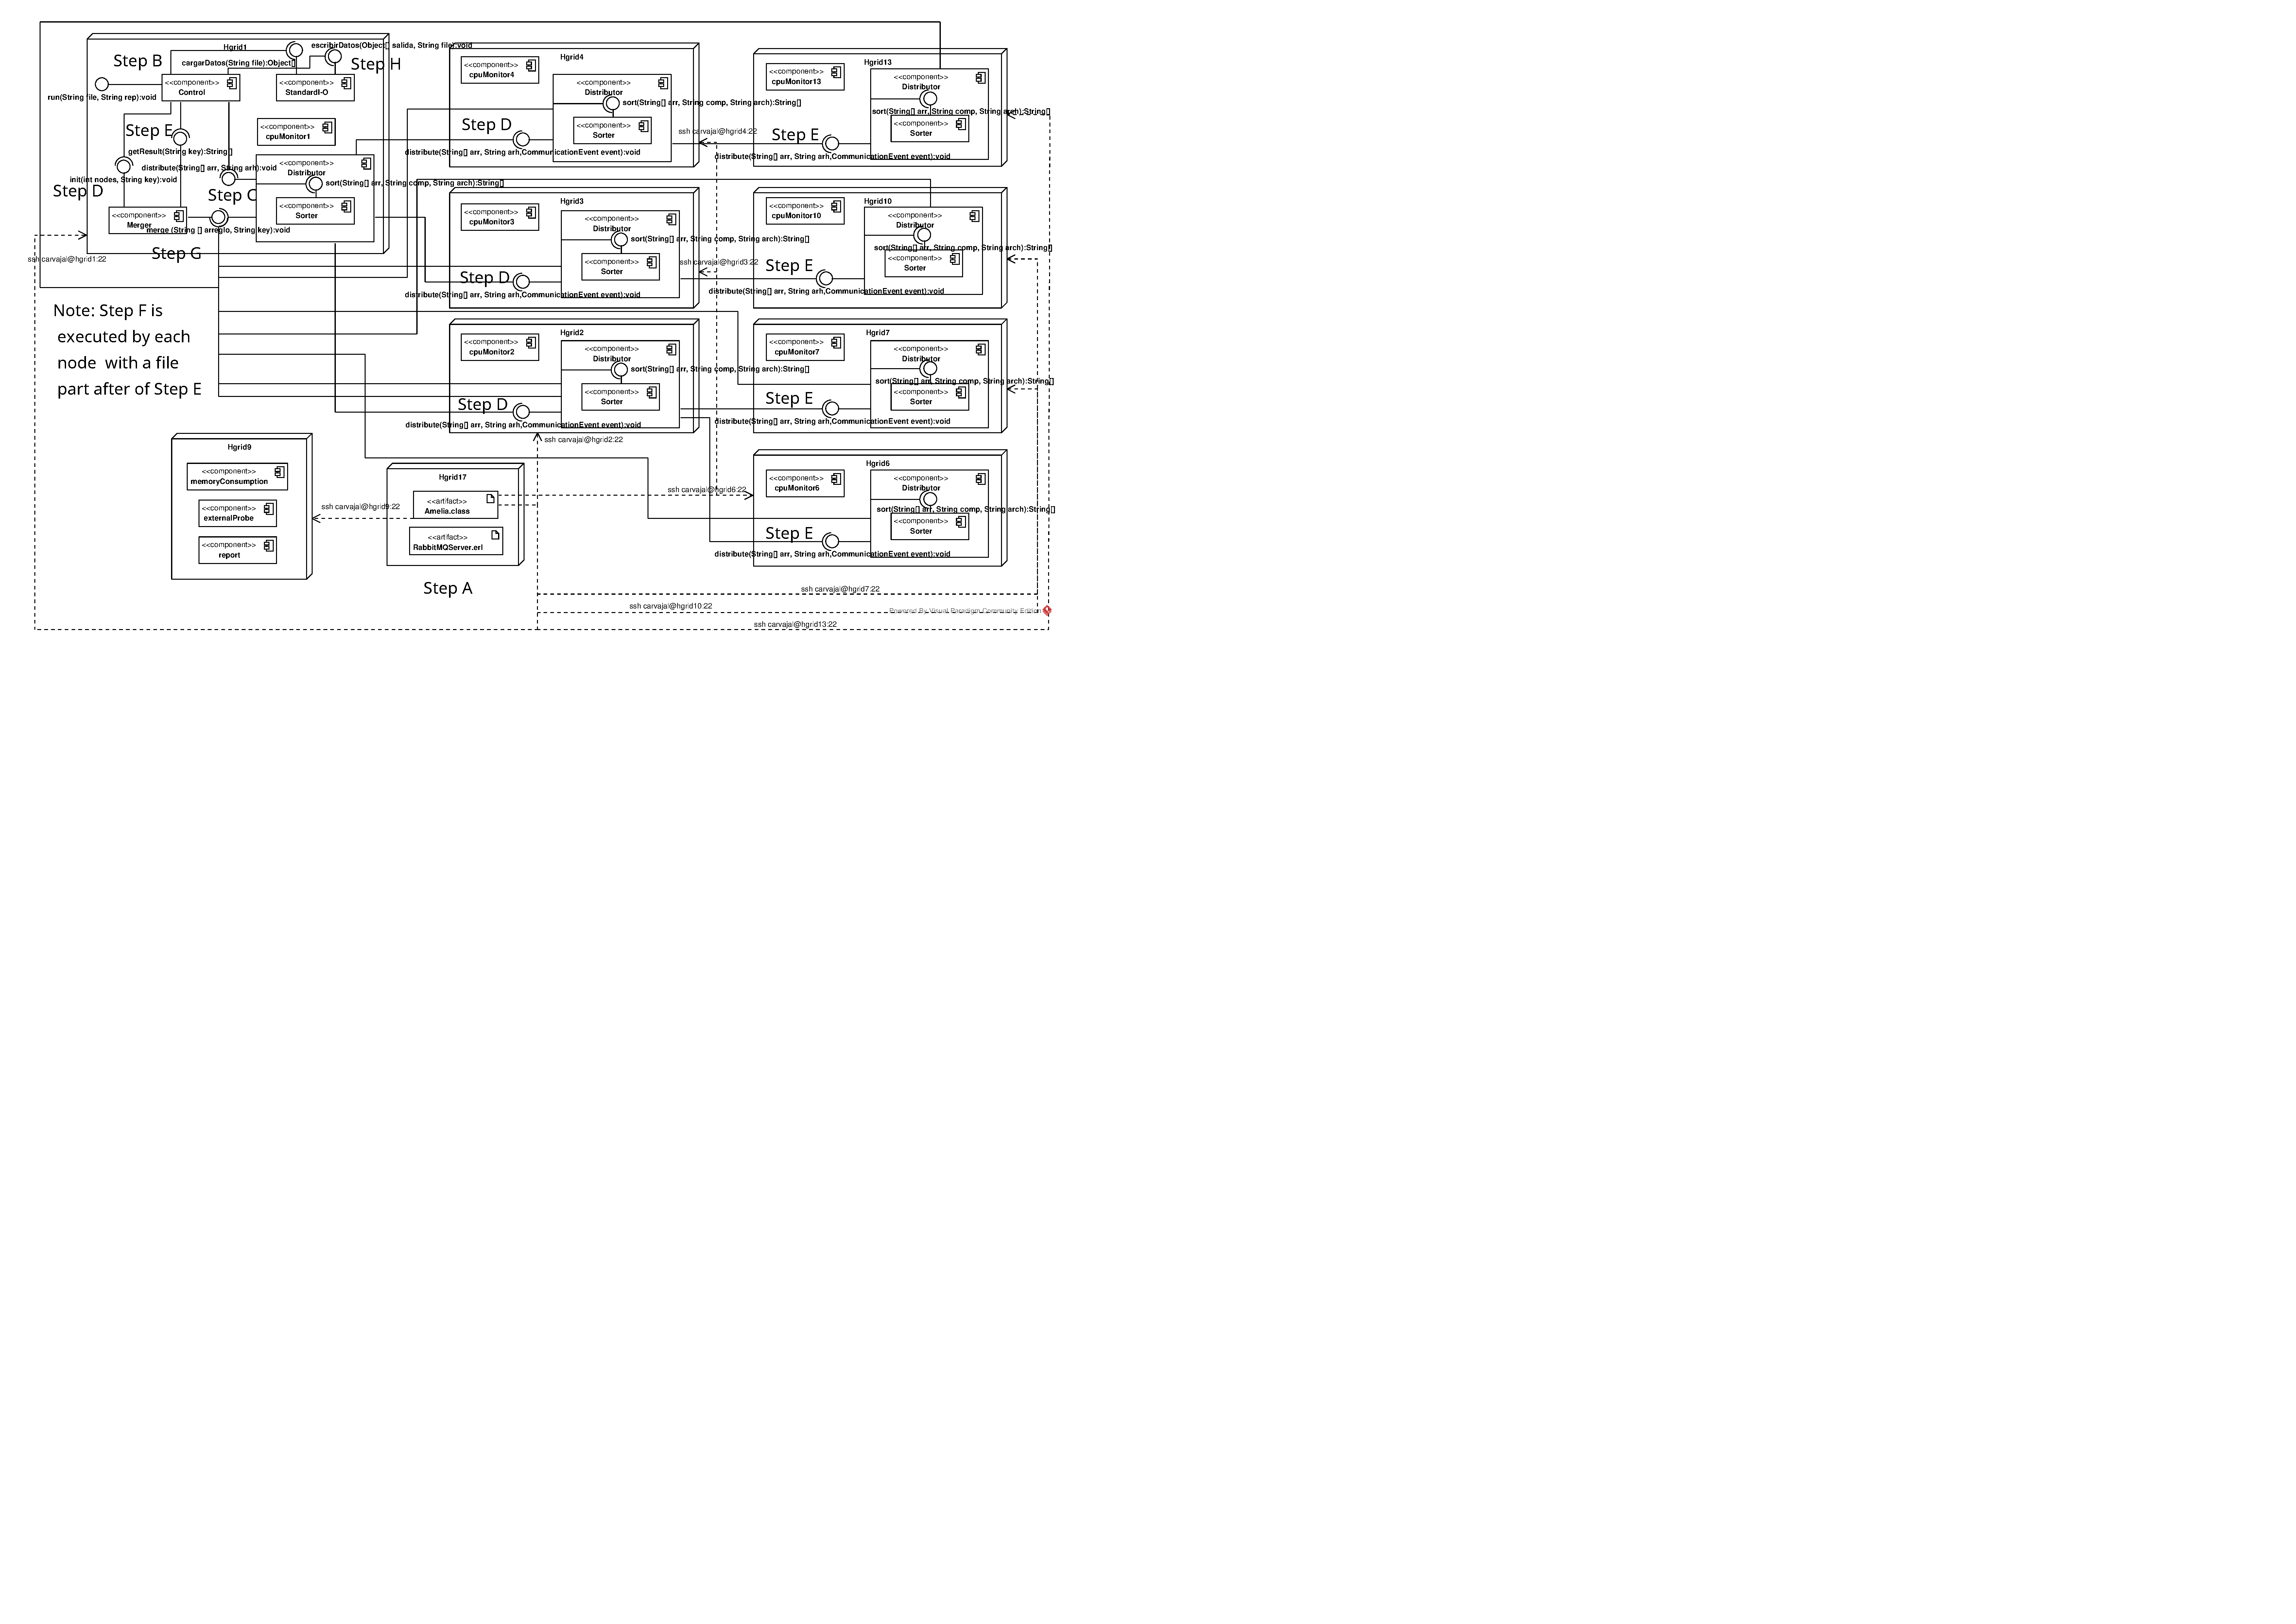
\includegraphics[trim=2cm 50cm -6cm 0cm, scale=0.46]{fig/JCMunozDistributedFJ.pdf}
		\caption{Amelia - Deployment Diagram - Fork-Join Design Pattern}
		\label{fig:diagramJCMunozDistributedFJ}
	\end{figure}
\end{landscape}

\subsubsection{Leader-Followers Design Pattern}
To implement this pattern in a distributed deployment for the sorting problem we assume three conditions. First, the asynchronous part of the pattern is realized by using threads to send requests, to simulate requests we split input data in chunks and each chunk is interpreted as a new request. Second, to avoid requests loss we implemented a request queue, which is responsible for storing requests when all processing nodes are busy. Third, to fulfill the threadpool functions we implement the LFManager component, which is responsible for managing the available processing nodes, assign them work, and manage their state changes (i.e., leader, follower, and processor). 

Figure \ref{fig:diagramJCMunozLeader-Followers} shows the deployment diagram specifying the application of this pattern.

The behavior of the Leader-Followers Design Pattern is described next:

\begin{description}
	\item [Step A] The Jmeter component of the processing node Hgrid17 starts processing when it calls the run method of the control component (processing node Hgrid1).
	\item [Step B] The control component sends to the StandardI-O component a read request to load the input file.
	\item [Step C] In this step two requests are sent. (i) the control component initializes the LFManager component; and (ii) the control component initializes the merger component.
	\item [Step D] In this step two requests are sent. (i) A new user request is registered in the queue component; and (ii) the control component sends to the merger component a request to get the whole sorted file when all file parts will be merged.
	\item [Step E] Sort requests (depending of the chunk size defined) of the user request are registered in the queue component.
	\item [Step F] The control component sends a request to the LFManager component to start the processing.
	\item [Step G] The LFManager component requests to the queue component for a sort request.
	\item [Step H] The LFManager component sends to the sorter leader component the sort request obtained from the queue component and selects a new sorter leader component. When the sort component finishes to process the sort request, it sends a request to the merge component which will merge all file parts.
	\item [Step I] The LFManager component requests to the queue component asking if there are sort requests for processing. If there are sort requests Step G, H and I are repeated until there are not sort requests to process.
	\item [Step J] The merger component receives all sorted file parts, it merges the whole sorted file and answers to the control component the request realized in Step D.
	\item [Step K] The control component receives the whole sorted file and it sends a write request to the StandardI-O component.
\end{description}

\begin{figure}[p!]
	\centering
	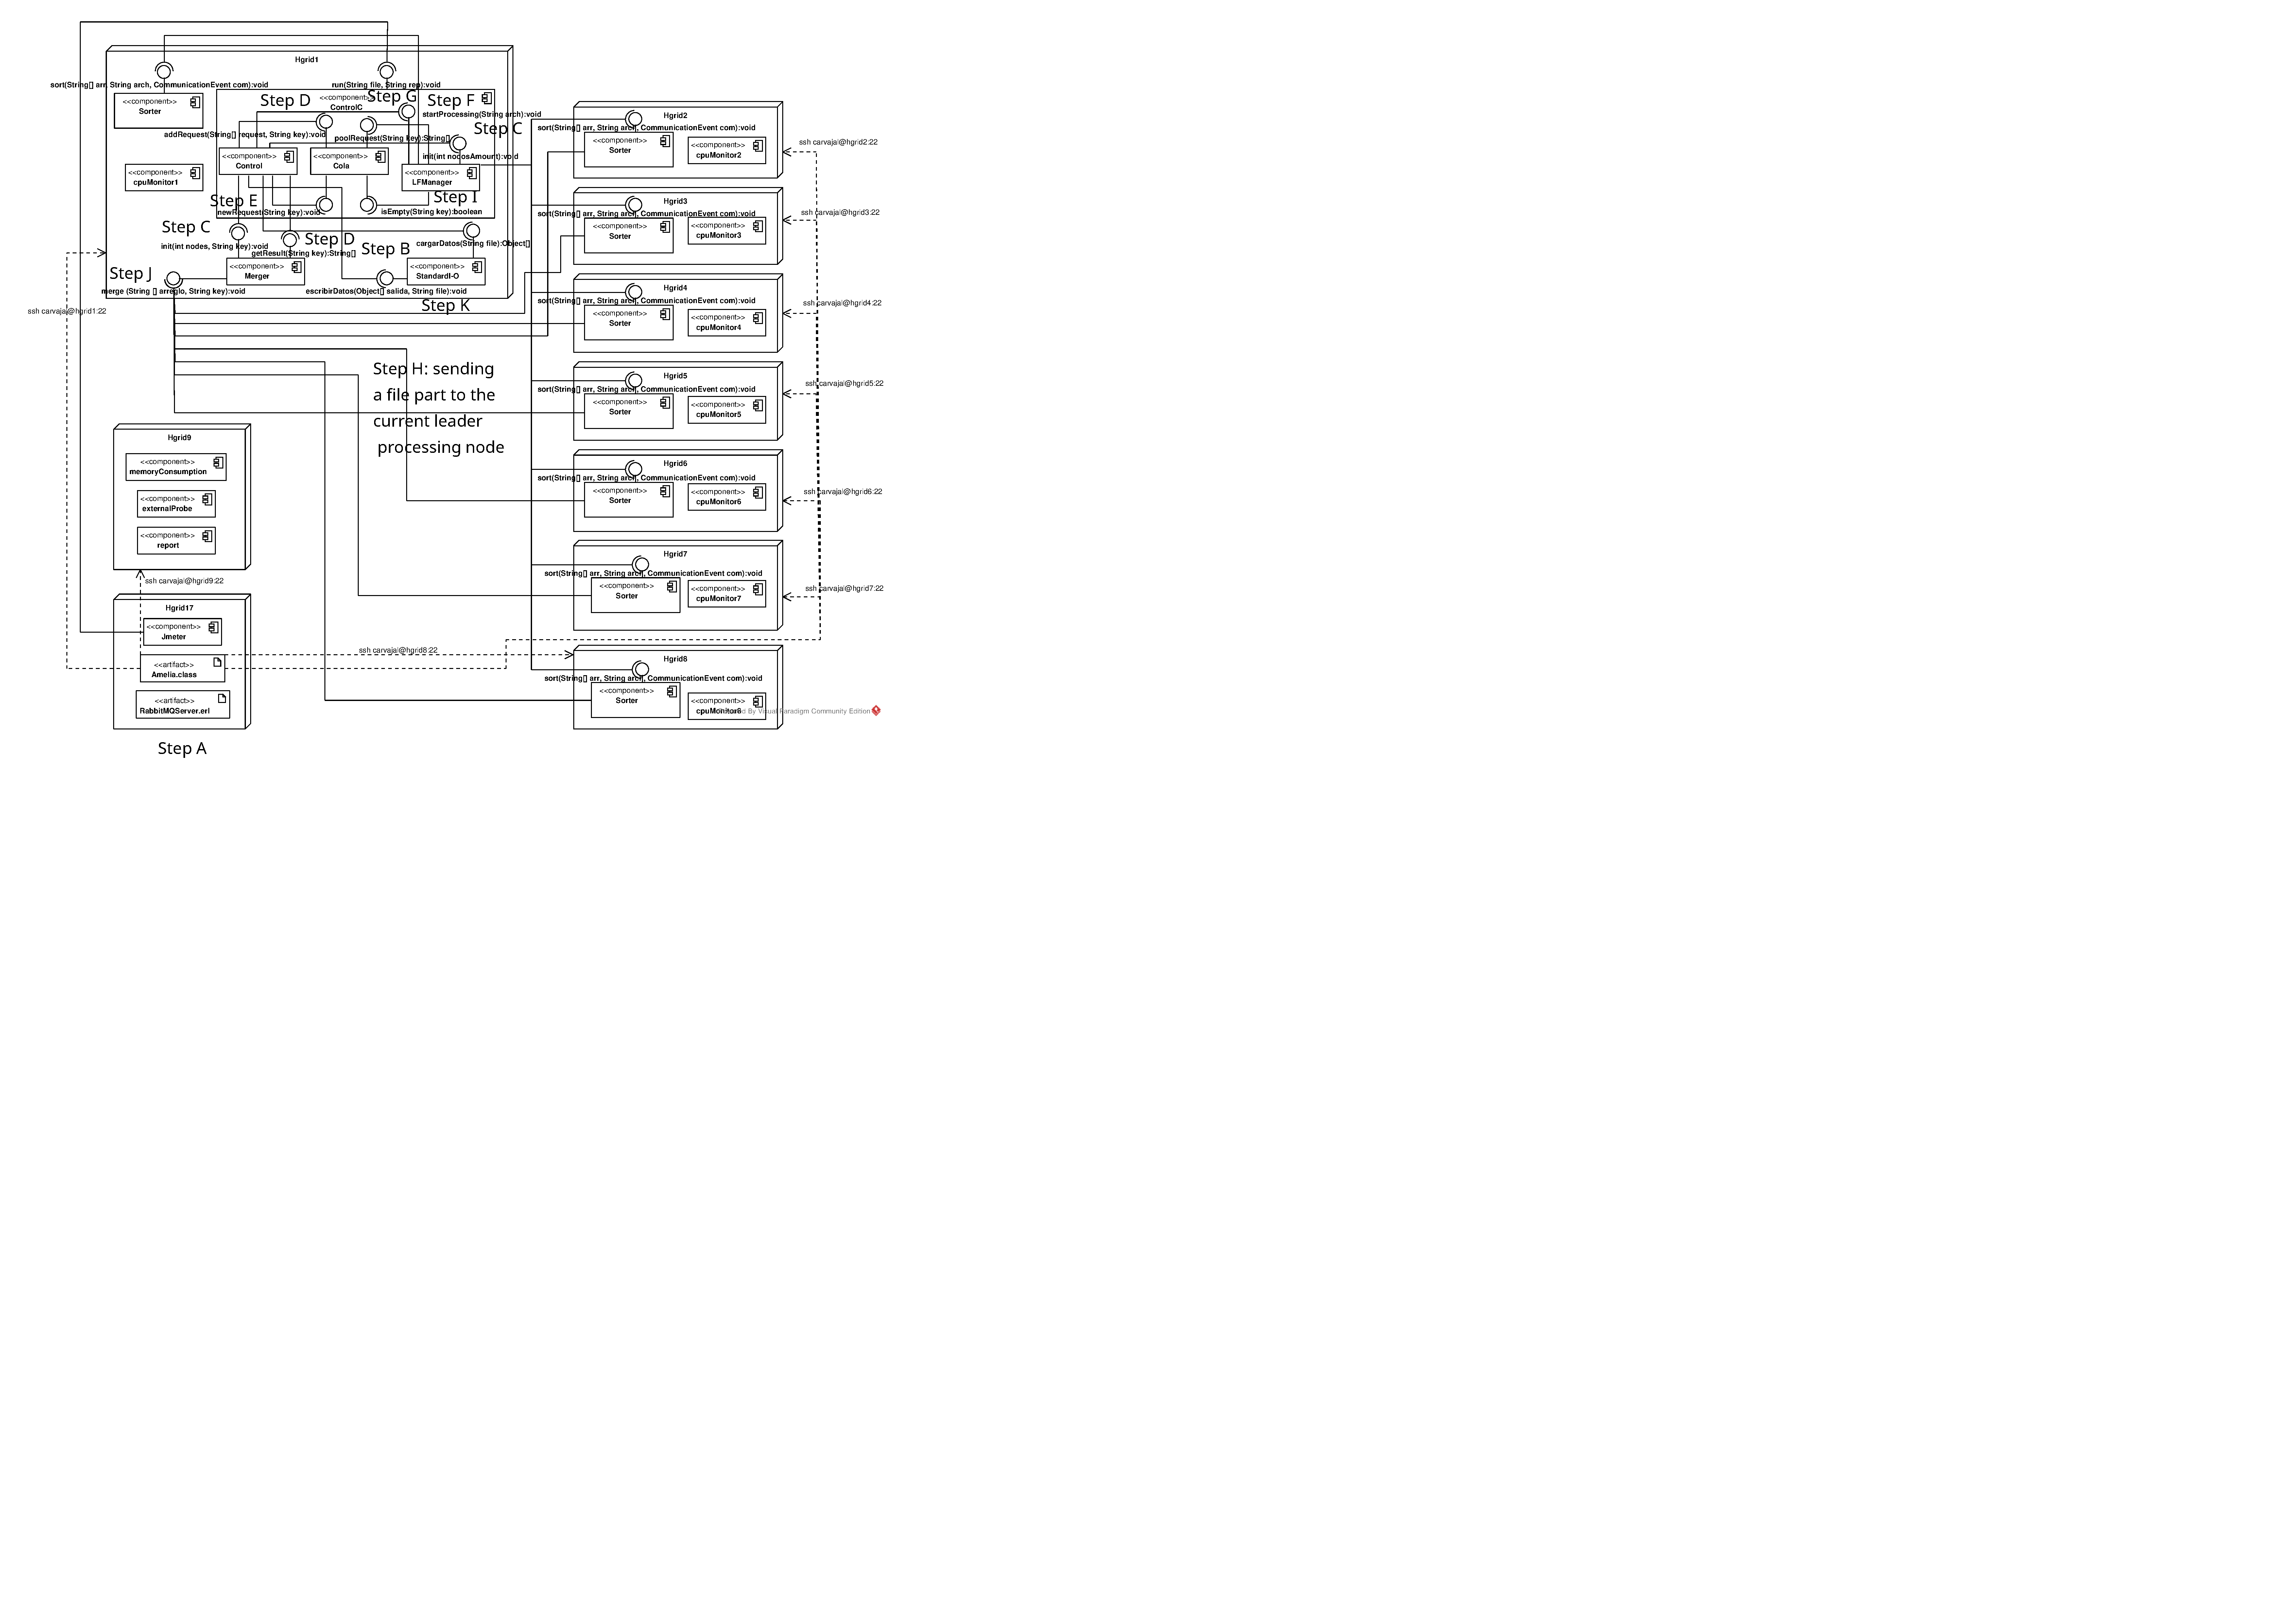
\includegraphics[trim=5cm 45cm -5cm 4cm, scale=0.45]{fig/JCMunozLeader-Followers.pdf}
	\caption{Amelia - Deployment Diagram - Leader-Followers Design Pattern}
	\label{fig:diagramJCMunozLeader-Followers}
\end{figure}

\section{Preparatory Experiments}
\label{sec:prepExperiments}
Prior to starting the execution of the designed experiments, there are two critical aspects to be defined: (i) how to distribute components along processing nodes? and (ii) which is the minimum problem size from which distribution is worth performing? These questions were proposed in previous chapter, and these must be answered before to start the experiment execution. Given that answer to these questions could vary according to each design pattern, we performed calibration experiments with each pattern.

The first question is focused mainly on locating the merge component and the components that are subsidiary to those closely related to the core solution components (i.e., Control and Standard I-O components). Components that complement experiments (i.e., probe and report components, deployment classes and the queued Server) are located in an additional node to minimize their performance effects in experiments.

The second question identifies a problem size that allows experiment results to be comparable among all design patterns and context variable scenarios, ensuring that a distributed deployment presents a better performance than in a single-machine deployment.

\subsection{Distribution of the Merge Component and the non-core System Components}
Sorting is usually solved through two phases: sort and merge. Our solution implements them in two main components, and given that we are working in a distributed deployment environment we use a third component responsible for distributing load work. Additional to our three main solution components we need two components more to sort one file: first, a component responsible for reading and writing the file, and second, a control manager component responsible for controlling interactions among all other components and receive user requests. 

Before executing the experiments, the location of each component in processing nodes must be defined (i.e., the software architecture of the system must be designed). Core components are: the Sort component responsible to sort the input file or a file part according to the Distributor component; the Distributor component, responsible to split the input file among processing nodes according to the available processing nodes; and the Merge component responsible to merge all the file parts to generate the result. Location of Sort and Distributor components is defined according to two variables: strategy or design pattern and the available processing nodes. As we mentioned before, we selected the next strategies and design patterns for our experiments: (i) the JC Sorting Strategy, (ii) the JC Sorting Strategy Variant, (iii) the Fork / Join design pattern and (iv) the Leader / Followers design pattern. Figures \ref{fig:diagramJCMunozOriStr}, \ref{fig:diagramJCMunozMergerSeparated}, \ref{fig:diagramJCMunozDistributedFJ}, and \ref{fig:diagramJCMunozLeader-Followers} determines components location of each pattern for a configuration with 8 available nodes.

The merge component is an special case because the original JC Sorting Strategy proposed one merge component for each sort component. Therefore, many merge phases were executed. However, given that merge has a complexity of O(n), having only one merge phase can improve performance. However, if there is only one merge component, where should it be located? we identify the next two possibilities (i) in the same processing node than the main distributor or (ii) in an additional processing node. For the non-core components, there are also many possible locations, and we identify the next ones (i) all non-core components in the same processing node than the main distributor (ii) each non-core component in an additional processing node, (iii) all non-core components in one additional processing node. However, option (ii) can introduce more latency and causing performance loss, thus this option was discarded.

For the remaining possible locations identified for the merge component and the non-core components, we executed calibration experiments where these components could be located in two ways, (i) all components in the same processing node than main distributor (ii) all components in an additional processing node. Table \ref{tab:optionsDescription} show these options and table \ref{tab:componentsLocation} show consolidated results of calibration experiments. Configurations 1, 2, 3 and 4 in table \ref{tab:componentsLocation} represent alternative options  of table \ref{tab:optionsDescription}. To analyze if the merge component and the non-core components should be located in an additional processing node or in the same processing node where the main distributor is located, we compared processing times using a monolithic (i.e., using only one sort component) and a distributed environments (i.e., using two sort components). For this analysis, we compared options 1 with 3 and 2 with 4 given that we first compare where we should locate components for each experiment environment. Table \ref{tab:componentsLocation} shows that in previous file sizes to highlighted cells, the option "all components in one additional processing node" is better, however, file sizes after highlighted cells are better with option "all components in the same processing node than main distributor" in both experiment environments, therefore, we decided to locate all additional components in the same processing node than the main distributor.

Other results that we observed in this experiment are: 

\begin{itemize}
	\item Comparing monolithic and distributed deployments, we can observe that depending on the used configuration the minimum file size to improve performance using distribution vary.
	\item The Norma memory structure has a better behavior than the Uma memory structure in monolithic environments and for the Fork/Join and Leader/Follower design patterns. The first observation can be explained given that these configurations do not add latency caused by access to remote data (i.e., data located in the NAS repository). The second observation must be analyzed with more experiments in the next chapter.
	\item The Leader/Followers pattern does not show a significant difference among experiments configurations, therefore, we will analyze its behavior in detail with more experiments in the next chapter.
	\item The Fork/Join design pattern improves performance in distributed deployment in almost all experiment scenarios from the most little file size. However, its performance, compared with other patterns or strategies, is the worst.
	\item The JC Sorting strategy variant and the Fork/Join Java library show the best performance in comparison with other patterns.
	\item We detect a limitation in the Norma memory structure in the monolithic deployment. In configuration where all components are located in the same processing node than the main distributor and using only one sort component (i.e., option 1) of the Fork/Join Java Library strategy we observe that from the $3'200.000$ file size, the experiments have an overload RAM memory. This overload causes a performance loss. This situation can be explained due to the memory resources consumed by all components containing additional replication of input data (i.e., local data).
\end{itemize}

% Please add the following required packages to your document preamble:
% \usepackage{graphicx}
\begin{table}[]
	\centering
	\caption{Options Description of Table \ref{tab:componentsLocation}}
	\label{tab:optionsDescription}
	\resizebox{0.5\textwidth}{!}{%
		\begin{tabular}{|c|c|}
			\hline
			\textbf{Option} & \textbf{Description} \\ \hline
			1 & \begin{tabular}[c]{@{}c@{}}All components in the same processing \\node than main distributor including only \\one sort component (Monolithic processing)\end{tabular} \\ \hline
			2 & \begin{tabular}[c]{@{}c@{}}All components in the same processing \\node than main distributor and using two \\sort components (Distributed processing)\end{tabular} \\ \hline
			3 & \begin{tabular}[c]{@{}c@{}}All components in an additional processing \\node including only one sort component \\(Monolithic processing)\end{tabular} \\ \hline
			4 & \begin{tabular}[c]{@{}c@{}}All components in an additional processing \\node and using two sort components \\(Distributed processing)\end{tabular} \\ \hline
		\end{tabular}%
	}
\end{table}

\subsection{Minimum File Size to Distribute Sorters}

To preserve comparability and to avoid executing irrelevant experiments, we executed preliminary experiments that answers the next question: Which is the minimum file size from which all selected design patterns can take advantage of distribution? Table \ref{tab:mimfileSizeEx} consolidates results of these experiments.

Results show that when the JC Sorting Strategy is configured with NORMA memory structure, it never improves their performance in a distributed deployment. In table \ref{tab:mimfileSizeEx}, for any file size used in this scenario, it can be observed that when the data is processed using 1 processing node (i.e., in the monolithic configuration) is better than using 2 processing nodes (i.e., in the distributed configuration). However, if the strategy is configured with the UMA memory structure, this strategy has a better performance in a distributed deployment in contrast to a monolithic configuration from first file size. Therefore, we decided not to execute more experiments with configuration of the JC Sorting Strategy with NORMA memory structure. 

According to the consolidated data in table \ref{tab:mimfileSizeEx}, the minimum file size from which an improvement is observed when the file is processed in a distributed environment is not uniform among all experiment scenarios. That is, each configuration can improve their performance in a distributed deployment from different file size. Highlighted cells show where each configuration starts to leverage distribution. Most of the highlighted cells are in the $200.000$ file size. However, to select the minimum file size for our experiments we decided to select a more representative minimum file size among all experiment scenarios. We take as the minimum file size that one with medium value among the largest three (i.e., $1'600.000$, $1'800.000$ and $2'200.000$). Therefore, $1'800.000$ lines is selected as the minimum file size.

In this experiment, the limitation observed in the RAM memory with the Norma memory structure in monolithic deployment in the previous experiment is also observed. This can be observed in configurations where all components are located in the same processing node that the main distributor and using only one sort component (i.e., option 1) of the Fork/Join Java Library strategy from the $3'200.000$ file size. After to analyze this behavior, we think that it is caused because in this point (file size  $3'200.000$) the RAM is overload due to the memory consumption of each component (i.e., middleware RAM requirements to deploy one component) and the file replication by each component to process their file part.

\begin{landscape}
	% Please add the following required packages to your document preamble:
	% \usepackage{multirow}
	% \usepackage{graphicx}
	% \usepackage[table,xcdraw]{xcolor}
	% If you use beamer only pass "xcolor=table" option, i.e. \documentclass[xcolor=table]{beamer}
	\begin{table}[]
		\fontsize{12}{24}\selectfont
		\centering
		\caption{Experiments for Locating Components (Latency in ms) }
		\label{tab:componentsLocation}
		\resizebox{1.45\textwidth}{!}{%
			\begin{tabular}{|c|c|c|c|c|c|c|c|c|c|c|c|c|c|c|c|c|c|c|c|c|c|c|c|c|c|c|c|c|c|c|c|c|}
				\hline
				& \multicolumn{8}{c|}{The JC Sorting Strategy Variation (ms)} & \multicolumn{8}{c|}{Fork/JoinJava library (ms)} & \multicolumn{8}{c|}{Fork-Join Design Pattern (ms)} & \multicolumn{8}{c|}{Leader-Followers Design Pattern (ms)} \\ \cline{2-33} 
				& \multicolumn{4}{c|}{Norma} & \multicolumn{4}{c|}{Uma} & \multicolumn{4}{c|}{Norma} & \multicolumn{4}{c|}{Uma} & \multicolumn{4}{c|}{Norma} & \multicolumn{4}{c|}{Uma} & \multicolumn{4}{c|}{Norma} & \multicolumn{4}{c|}{Uma} \\ \cline{2-33} 
				\multirow{-3}{*}{File Size} & 1 & 2 & 3 & 4 & 1 & 2 & 3 & 4 & 1 & 2 & 3 & 4 & 1 & 2 & 3 & 4 & 1 & 2 & 3 & 4 & 1 & 2 & 3 & 4 & 1 & 2 & 3 & 4 & 1 & 2 & 3 & 4 \\ \hline
				200.000 & 464 & 1426 & 488 & 1439 & 1423 & 804 & 1433 & 1197 & 926 & 1865 & 946 & 1868 & 1986 & 1636 & 1921 & 1303 & 937 & 965 & 1002 & 968 & \cellcolor{yellow}1968 & 1959 & \cellcolor{yellow}1994 & 1931 & 561 & 551 & 520 & 547 & \cellcolor{yellow}1425 & \cellcolor{yellow}1529 & \cellcolor{yellow}1495 & \cellcolor{yellow}1514 \\ \hline
				400.000 & 923 & 1799 & 937 & 1804 & 2831 & \cellcolor{yellow}1539 & 2791 & \cellcolor{yellow}1936 & 1378 & 2206 & 1386 & 2156 & 3452 & \cellcolor{yellow}2324 & 3226 & \cellcolor{yellow}2692 & 1917 & 2291 & 1936 & 1894 & 3848 & \cellcolor{yellow}3877 & 3959 & \cellcolor{yellow}3918 & \cellcolor{yellow}1085 & \cellcolor{yellow}1067 & \cellcolor{yellow}1113 & \cellcolor{yellow}1125 & 2777 & 3042 & 2790 & 3157 \\ \hline
				600.000 & 1475 & 2203 & 1489 & 2189 & 4241 & 2655 & 4202 & 2406 & 1810 & 2470 & 1799 & 2494 & 4930 & 2604 & 4532 & 2661 & 3473 & \cellcolor{yellow}3158 & 3444 & \cellcolor{yellow}3475 & 6326 & 3411 & 6495 & 4326 & 1668 & 1613 & 1633 & 1698 & 4177 & 4540 & 5117 & 4664 \\ \hline
				800.000 & 1953 & 2618 & 1925 & 2551 & 5715 & 3076 & 5641 & 3430 & 2176 & 2726 & 2165 & 2758 & 6241 & 3264 & 5840 & 3659 & 3816 & 3513 & 3869 & 3894 & 7705 & 4076 & 7842 & 4162 & 2202 & 2210 & 2220 & 2283 & 5554 & 6079 & 5709 & 6130 \\ \hline
				1'000.000 & 2418 & 2955 & 2356 & 2945 & 7078 & 3894 & 7012 & 3835 & 2548 & 3257 & 2511 & 3234 & 7673 & 4079 & 7081 & 4468 & 6392 & 4874 & 6376 & 6430 & 11158 & 6308 & 11650 & 6684 & 2827 & 2743 & 2755 & 2832 & 6999 & 7700 & 7347 & 7663 \\ \hline
				1'200.000 & 3095 & 3568 & 3126 & 3526 & 8768 & 5011 & 8595 & 5370 & 3196 & 3733 & 3183 & 3764 & 9181 & 4921 & 8517 & 5291 & \cellcolor{yellow}7067 & 5463 & \cellcolor{yellow}7129 & 7062 & 12823 & 7415 & 13168 & 6867 & 3478 & 3417 & 3435 & 3534 & 8464 & 9236 & 9144 & 9263 \\ \hline
				1'400.000 & 3692 & 3911 & 3623 & 3916 & 10078 & 5443 & 10031 & 5920 & 3578 & 4040 & 3548 & 3939 & 10656 & 5580 & 9899 & 5668 & 7452 & 5868 & 7530 & 7525 & 14144 & 8268 & 14661 & 7935 & 4024 & 3975 & 4010 & 4136 & 10138 & 10788 & 10692 & 10869 \\ \hline
				1'600.000 & 4233 & 4403 & 4082 & 4362 & 11627 & 6263 & 11402 & 6201 & 4050 & 4478 & 3936 & 4274 & 12105 & 6376 & 11274 & 6330 & 8031 & 6235 & 7965 & 8013 & 15580 & 9008 & 16109 & 8704 & 4654 & 4605 & 4778 & 4985 & 11277 & 12405 & 12647 & 12474 \\ \hline
				1'800.000 & 4844 & 4817 & 4669 & 4747 & \cellcolor{yellow}13062 & 6964 & \cellcolor{yellow}13102 & 7252 & 4544 & 4808 & 4468 & 4732 & 13498 & 7056 & 12931 & 7634 & 12682 & 8911 & 12754 & 12662 & 21470 & 12420 & 22055 & 11512 & 5310 & 5393 & 5328 & 5538 & 12845 & 13955 & 13380 & 13993 \\ \hline
				2'000.000 & \cellcolor{yellow}5385 & \cellcolor{yellow}5283 & \cellcolor{yellow}5548 & \cellcolor{yellow}5327 & 14611 & 7962 & 14931 & 7980 & \cellcolor{yellow}4975 & \cellcolor{yellow}5195 & \cellcolor{yellow}5317 & \cellcolor{yellow}5270 & 14992 & 8046 & 14039 & 8445 & 13318 & 9219 & 13198 & 13168 & 22608 & 12456 & 23537 & 12895 & 6049 & 6009 & 6012 & 6335 & 14394 & 15684 & 15774 & 15786 \\ \hline
				2'200.000 & 6479 & 6169 & 6824 & 6372 & 16200 & 8923 & 16780 & 9373 & 5873 & 5832 & 6333 & 5838 & 16873 & 8481 & 15843 & 9425 & 14258 & 10131 & 14430 & 14470 & 24405 & 13759 & 25210 & 13658 & 6809 & 6838 & 7143 & 7370 & 15965 & 17556 & 18047 & 17856 \\ \hline
				2'400.000 & 6864 & 6634 & 7203 & 6784 & 17656 & 9617 & 18123 & 9707 & 6443 & 6153 & 6739 & 6125 & 18247 & 9276 & 17197 & 10084 & 14684 & 10477 & 15012 & 14899 & 25910 & 14240 & 26934 & 14504 & 7499 & 7592 & 7729 & 7998 & 17561 & 19040 & 19072 & 19290 \\ \hline
				2'600.000 & 7669 & 7074 & 7884 & 7451 & 18909 & 10347 & 19462 & 10803 & 6998 & 6598 & 7651 & 6602 & 19658 & 10334 & 18724 & 10742 & 15517 & 11086 & 15625 & 15623 & 27126 & 15290 & 28095 & 16093 & 8446 & 8444 & 8827 & 8880 & 19252 & 20642 & 20460 & 21010 \\ \hline
				2'800.000 & 8244 & 7659 & 8515 & 7979 & 20591 & 11185 & 20844 & 11136 & 7640 & 7194 & 7780 & 7348 & 20906 & 10813 & 19898 & 11434 & 15962 & 11532 & 16024 & 16055 & 28516 & 16430 & 29729 & 16023 & 9165 & 9072 & 9239 & 9676 & 20328 & 22391 & 22121 & 22750 \\ \hline
				3'000.000 & 8871 & 8072 & 9264 & 9010 & 21977 & 11856 & 22723 & 12613 & 8064 & 7458 & 8659 & 7777 & 22431 & 11699 & 21966 & 12114 & 16759 & 12308 & 16789 & 17034 & 30219 & 16327 & 31070 & 17311 & 9852 & 9869 & 9925 & 10455 & 21754 & 24070 & 24108 & 24520 \\ \hline
				3'200.000 & 9523 & 8694 & 9670 & 8918 & 23497 & 12615 & 23924 & 13076 & \cellcolor{lightgray}31630 & 7885 & 8809 & 8231 & 23897 & 12033 & 22919 & 12743 & 17140 & 12577 & 17164 & 17440 & 31611 & 17268 & 32486 & 17521 & 10656 & 10557 & 10993 & 11186 & 23501 & 25602 & 25180 & 25886 \\ \hline
				3'400.000 & 10113 & 9097 & 10639 & 9122 & 24986 & 13445 & 25406 & 14222 & \cellcolor{lightgray}61993 & 8054 & 9866 & 8125 & 25286 & 12451 & 24588 & 14336 & 26349 & 17695 & 26747 & 26619 & 42282 & 23535 & 43747 & 23866 & 11423 & 11325 & 11365 & 12005 & 24878 & 27470 & 26567 & 27867 \\ \hline
				3'600.000 & 10495 & 9543 & 10920 & 9765 & 26362 & 14464 & 27436 & 15062 & \cellcolor{lightgray}18039 & 9142 & 9978 & 9559 & 26873 & 14827 & 25791 & 15513 & 26975 & 18112 & 27103 & 26973 & 43677 & 23684 & 45173 & 24952 & 12012 & 12077 & 12032 & 12423 & 26430 & 28969 & 28841 & 29456 \\ \hline
				3'800.000 & 11015 & 9994 & 11566 & 10499 & 27957 & 15292 & 28872 & 16381 & \cellcolor{lightgray}17897 & 10093 & 11233 & 10130 & 28383 & 14607 & 27181 & 15937 & 29124 & 18596 & 27852 & 27930 & 45059 & 25153 & 46789 & 25351 & 12901 & 12808 & 12801 & 13404 & 28344 & 30988 & 30932 & 31379 \\ \hline
				4'000.000 & 11873 & 10582 & 11788 & 10875 & 29674 & 16549 & 30502 & 16887 & \cellcolor{lightgray}76094 & 11536 & 11119 & 9864 & 29623 & 15589 & 28483 & 16421 & 43984 & 19495 & 28213 & 28622 & 46591 & 25988 & 48440 & 25896 & 13424 & 13540 & 13931 & 13985 & 29443 & 32340 & 33703 & 33259 \\ \hline
			\end{tabular}%
		}
	\end{table}
\end{landscape}

\begin{landscape}
	% Please add the following required packages to your document preamble:
	% \usepackage{multirow}
	% \usepackage{graphicx}
	\begin{table}[]
		\fontsize{10}{18}\selectfont
		\textmd
		\centering
		\caption{Minimum File Size Experiment}
		\label{tab:mimfileSizeEx}
		\resizebox{1.4\textwidth}{!}{%
			\begin{tabular}{|c|c|c|c|c|c|c|c|c|c|c|c|c|c|c|c|c|c|c|c|c|}
				\hline
				\multirow{3}{*}{\begin{tabular}[c]{@{}c@{}}File\\   Size\end{tabular}} & \multicolumn{4}{c|}{The JC Sorting Strategy} & \multicolumn{4}{c|}{The JC Sorting Variation} & \multicolumn{4}{c|}{Fork/Join Java library} & \multicolumn{4}{c|}{Fork-Join Design Pattern} & \multicolumn{4}{c|}{Leader-Followers Design Pattern } \\ \cline{2-21} 
				& \multicolumn{2}{c|}{NORMA} & \multicolumn{2}{c|}{UMA} & \multicolumn{2}{c|}{NORMA} & \multicolumn{2}{c|}{UMA} & \multicolumn{2}{c|}{NORMA} & \multicolumn{2}{c|}{UMA} & \multicolumn{2}{c|}{NORMA} & \multicolumn{2}{c|}{UMA} & \multicolumn{2}{c|}{NORMA} & \multicolumn{2}{c|}{UMA} \\ \cline{2-21} 
				& 1 & 2 & 1 & 2 & 1 & 2 & 1 & 2 & 1 & 2 & 1 & 2 & 1 & 2 & 1 & 2 & 1 & 2 & 1 & 2 \\ \hline
				200.000 & 436 & 469 & \cellcolor{yellow}1360 & \cellcolor{yellow}832 & 464 & 1426 & \cellcolor{yellow}1423 & \cellcolor{yellow}804 & 926 & 1865 & \cellcolor{yellow}1986 & \cellcolor{yellow}1636 & 937 & 965 & 1968 & 1959 & \cellcolor{yellow}561 & \cellcolor{yellow}551 & 1425 & 1529 \\ \hline
				400.000 & 776 & 864 & 2613 & 1587 & 923 & 1799 & 2831 & 1539 & 1378 & 2206 & 3452 & 2324 & 1917 & 2291 & 3848 & 3877 & 1085 & 1067 & 2777 & 3042 \\ \hline
				600.000 & 1299 & 1364 & 3905 & 2381 & 1475 & 2203 & 4241 & 2655 & 1810 & 2470 & 4930 & 2604 & \cellcolor{yellow}3473 & \cellcolor{yellow}3158 & \cellcolor{yellow}6326 & \cellcolor{yellow}3411 & 1668 & 1613 & 4177 & 4540 \\ \hline
				800.000 & 1630 & 1829 & 5224 & 3149 & 1953 & 2618 & 5715 & 3076 & 2176 & 2726 & 6241 & 3264 & 3816 & 3513 & 7705 & 4076 & 2202 & 2210 & 5554 & 6079 \\ \hline
				1.000.000 & 2108 & 2276 & 6489 & 3935 & 2418 & 2955 & 7078 & 3894 & 2548 & 3257 & 7673 & 4079 & 6392 & 4874 & 11158 & 6308 & 2827 & 2743 & 7074 & 7030 \\ \hline
				1.200.000 & 2779 & 2954 & 7857 & 4797 & 3095 & 3568 & 8768 & 5011 & 3196 & 3733 & 9181 & 4921 & 7067 & 5463 & 12823 & 7415 & 3478 & 3417 & 8623 & 8619 \\ \hline
				1.400.000 & 3134 & 3550 & 9177 & 5623 & 3692 & 3911 & 10078 & 5443 & 3578 & 4040 & 10656 & 5580 & 7452 & 5868 & 14144 & 8268 & 4024 & 3975 & 9993 & 10050 \\ \hline
				1.600.000 & 3703 & 3965 & 10532 & 6375 & 4233 & 4403 & 11627 & 6263 & 4050 & 4478 & 12105 & 6376 & 8031 & 6235 & 15580 & 9008 & 4654 & 4605 & \cellcolor{yellow}11473 & \cellcolor{yellow}11447 \\ \hline
				1.800.000 & 4167 & 4895 & 11847 & 7204 & \cellcolor{yellow}4844 & \cellcolor{yellow}4817 & 13062 & 6964 & 4544 & 4808 & 13498 & 7056 & 12682 & 8911 & 21470 & 12420 & 5310 & 5393 & 12843 & 12935 \\ \hline
				2.000.000 & 4666 & 5274 & 13301 & 7973 & 5385 & 5283 & 14611 & 7962 & 4975 & 5195 & 14992 & 8046 & 13318 & 9219 & 22608 & 12456 & 6049 & 6009 & 14249 & 14612 \\ \hline
				2.200.000 & 5520 & 6255 & 14780 & 8928 & 6479 & 6169 & 16200 & 8923 & \cellcolor{yellow}5873 & \cellcolor{yellow}5832 & 16873 & 8481 & 14258 & 10131 & 24405 & 13759 & 6809 & 6838 & 15881 & 15952 \\ \hline
				2.400.000 & 11167 & 8710 & 16077 & 9751 & 6864 & 6634 & 17656 & 9617 & 6443 & 6153 & 18247 & 9276 & 14684 & 10477 & 25910 & 14240 & 7499 & 7592 & 17291 & 17530 \\ \hline
				2.600.000 & 32477 & 33541 & 17446 & 10542 & 7669 & 7074 & 18909 & 10347 & 6998 & 6598 & 19658 & 10334 & 15517 & 11086 & 27126 & 15290 & 8446 & 8444 & 18810 & 18854 \\ \hline
				2.800.000 & 29485 & 40926 & 18745 & 11340 & 8244 & 7659 & 20591 & 11185 & 7640 & 7194 & 20906 & 10813 & 15962 & 11532 & 28516 & 16430 & 9165 & 9072 & 20185 & 20323 \\ \hline
				3.000.000 & 36953 & 117483 & 20078 & 12172 & 8871 & 8072 & 21977 & 11856 & 8064 & 7458 & 22431 & 11699 & 16759 & 12308 & 30219 & 16327 & 9852 & 9869 & 21411 & 21744 \\ \hline
				3.200.000 & 38117 & 206397 & 21387 & 13010 & 9523 & 8694 & 23497 & 12615 & \cellcolor{lightgray}31630 & 7885 & 23897 & 12033 & 17140 & 12577 & 31611 & 17268 & 10656 & 10557 & 22859 & 23042 \\ \hline
				3.400.000 & 271451 & 240498 & 22851 & 13629 & 10113 & 9097 & 24986 & 13445 & \cellcolor{lightgray}61993 & 8054 & 25286 & 12451 & 26349 & 17695 & 42282 & 23535 & 11423 & 11325 & 24941 & 25139 \\ \hline
				3.600.000 & 44432 & 292747 & 24287 & 14571 & 10495 & 9543 & 26362 & 14464 & \cellcolor{lightgray}18039 & 9142 & 26873 & 14827 & 26975 & 18112 & 43677 & 23684 & 12012 & 12077 & 26220 & 26417 \\ \hline
				3.800.000 & 65956 & 423089 & 25669 & 15465 & 11015 & 9994 & 27957 & 15292 & \cellcolor{lightgray}17897 & 10093 & 28383 & 14607 & 29124 & 18596 & 45059 & 25153 & 12901 & 12808 & 27598 & 28020 \\ \hline
				4.000.000 & 191262 & 551244 & 27053 & 16363 & 11873 & 10582 & 29674 & 16549 & \cellcolor{lightgray}76094 & 11536 & 29623 & 15589 & 43984 & 19495 & 46591 & 25988 & 13424 & 13540 & 28854 & 29209 \\ \hline
			\end{tabular}%
		}
	\end{table}
\end{landscape}

%\subsection{Batch Size to Fork/Join and Leader/Followers Design Patterns}%

\section{Control Tests}
\label{sec:controlTest}

To ensure that our experiments are not affected by unknown or irrelevant variables, we executed the same test repeatedly during a whole day. This is a control and calibration test. In this test, we expected no atypical results that suggest that there are environment variables which can affect our experiments.

Test was executed 4000 times. Execution time varied between 8038 and 9532 milliseconds, that is a range of 1494 milliseconds. This variation suggests that there are not other variables that affect our experiments. Figure \ref{fig:pruebaControl} also shows this test results.

Additionally, the configuration described in section \ref{sec:confandControl} was tested, and we observe that results were the expected, that is, this test was executed in the expected time range. If results were not between the expected results, we would have calibrated the configuration until achieving the expected results.

\begin{landscape}
	\begin{figure}[p!]
		\centering
		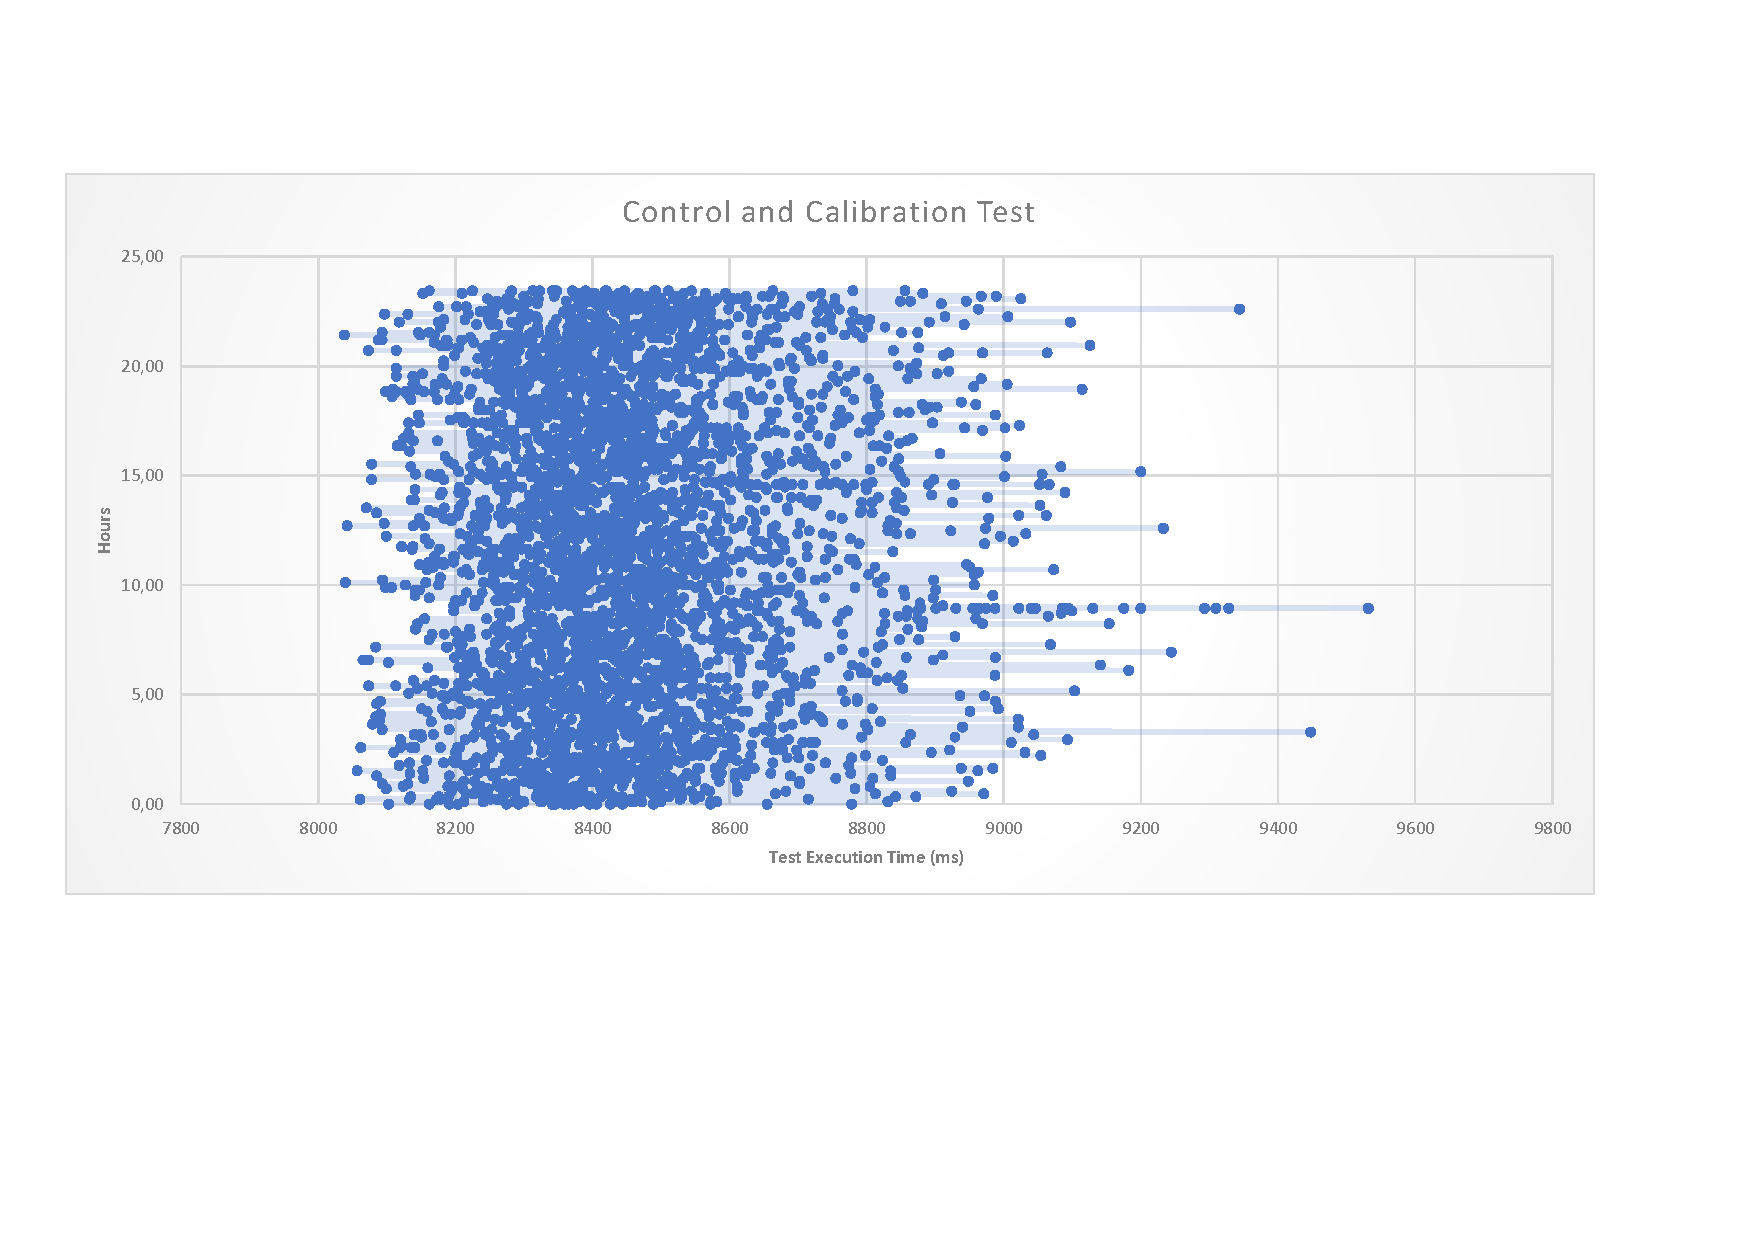
\includegraphics[trim=1cm 5cm 5cm 1cm, scale=0.9]{fig/PruebaControl.pdf}
		\caption{Control Tests Graph}
		\label{fig:pruebaControl}
	\end{figure}
\end{landscape}

\section{Experiments Execution}
Using the Amelia class files we automated the tests execution: in total, this amounts to 2535 experiments for the latency analysis and 324 for the throughput. The Liason laboratory was used during 24 hours for approximately two months with short pauses each two days.

For the throughput analysis, we decided to use only the four best configurations selected among the latency analysis. Additionally, only 11 different file sizes used, from $1'800.000$ lines until $9'800.000$ lines adding $800.000$ lines to each file. The experiments were repeated two times and results averaged, due to in the throughput experiments could exist little variations because many requests are sent at the same time and we did not control to send and neither arrive sequence.

The experiments results will be analyzed in the next chapter.

\section{Chapter Summary}
In this chapter, we executed the experiments designed in the before chapter. To execute these experiments we required to follow the next phases: first, we configured and controlled items like hardware, operating system, precision time protocol (it coordinates the time among the processing units to ensure the reliability in the taken measurements), among others. Second, we defined the software deployment configuration. Third, we executed preparatory experiments to define invariant values to execute all experiments like the minimum problem size and the additional component distribution. Fourth, we executed a control test to validate that there are not variables that can affect the experiment's measurements and results. And finally, we executed the experiments.








